\chapter{Литературный обзор}%
\label{cha:Литературный обзор}
\section{Гексагональный нитрид бора}%
\label{sec:Гексагональный нитрид бора}

Гексагональный нитрида бора (h-BN) по своей структуре аналог графита, поэтому
иногда называют "белым графитом". Кристаллическая структура h-BN представляет
из себя набор графеноподобных слоев, расположенных, в отличие от структуры 
графита точно один под другим с чередованием атомов B и N по оси Z. Расстояние 
между слоями в решетке нитрида бора равно 3,34 А, которое меньше, чем у графита
(3,40 А), что доказывает о более прочной связи между слоями в структуре BN.

Температура плавления h-BN под давлением азота больше 3000 °С, плотность 
составляет \SI{2.3}{\gram\per\cm^3} Гексагональный BN обладает полупроводниковыми свойствами
(с шириной запрещенной зоны около 3,7 эВ), так же обладает люминесцентными 
свойствами при наличии небольшого количества примесей. Нитрид бора при 
комнатной температуре химически инертен, он практически не реагирует с 
кислородом или хлором, кислотами или щелочами. Подвергается действию кислорода 
и хлора при температурах выше 700 °С. Вступает в реакцию с фтором (образуя \ce{BF3} 
и \ce{N2}) и с HF (образуя \ce{NH4BF4}); горячие растворы щелочей разлагают его с 
выделением \ce{NH3}.

Нитрид бора обладает превосходными антифрикционными свойствами. Нанопорошки
а так же покрытия нитрида бора широко используются в качестве сухой смазки [].
Данная особенность связана с сильной ковалентной связью между B - N базовой плоскости 
связанных между собой слабой Ван-дер-Ваальсой связью [].

\subsection{Методы получения гексагонального нитрида бора}%
\label{sub:Методы получения гексагонального нитрида бора}


Широко распространены следующие методы синтеза гексагонального нитрида бора:

\begin{itemize}
    \item Плазмотермический
    \item Метод СВС
    \item Методы химического осаждения
    \item Методы прямого синтеза
\end{itemize}

В самом общем случае синтез нитрида бора происходит по простой реакции \ce{B + N2}, 
которая может быть осуществлена в трубчатой печи сопротивления. Однако энергия, которую 
необходимо затратить на активацию молекулы \ce{Na} достаточно высока [конкретное
значение], а технологические требования к морфологии и структуре материала ставят
задачи по поиску новых, оптимальных методик по синтезу различных структур. 

\subsection{Газовое восстановление}%
\label{sub:Газовое востановление}

Первые исследовательские работы по изучению синтеза гексагонального BN учитывали
необходимость замены реагентов на прекурсоры с  меньшей энергией активации для 
прохождения реакции. Одним из решений может являться
замена \ce{N2} на \ce{NH4}, а чистого аморфного бора на \ce{H3BO3}. Первые
работы в области синтеза BN структур показали образование различных переходных 
продуктов: \ce{(B2O3)nNH} при \SI{200}{\degreeCelsius},
\ce{(BN)x(B2O3)y(NH3)z} при \SI{350}{\degreeCelsius}
\cite[]{economy_boron_1967}. Образование оксида бора с точкой плавления
\SI{450}{\degreeCelsius} приводит уменьшению удельной поверхности при
температурах выше температуры плавления, что приводит к агломерации
капель оксида бора и уменьшению контактной поверхности между реакционным
газом и прекурсором. Подобный эффект негативно сказывается на диффузии реакционного
газа через прекурсор, в результате чего в продуктах реакции наблюдается большое 
количество непрореагировавших реагентов, а так же полупродуктов. Чтобы преодолеть
данное технологическое ограничение синтез проводился в несколько этапов: синтез
в протоке реакционного газа прерывался, полупродукт перемалывался, далее синтез
возобновляли. Так же существенным технологическим осложнением являлось 
использование аммиака в качестве источника атомарного азота.

Для решения данной проблемы обычно используют инертные наполнители или
продукты реакции, которые не реагируют с исходными компонентами и газовой
средой, а так же не дают мельчайшим каплям оксида бора сливаться. И тут
возникает некоторая дилемма. С одной стороны, использование в качестве
наполнителя продукта реакции должно увеличивать чистоту выходящих
продуктов. Однако, в одной из первых работ, было показано что
использование альтернативных наполнителей (например ортофосфата кальция)
значительно увеличивает долю выхода BN в отношении к полупродуктам
\cite[]{basu_synthesis_1990}. С другой, использование альтернативных
наполнителей приводит к появлению дополнительных операций очистки BN от
примесей. Так же оставалась проблема синтеза частиц BN контролируемой
размерности и морфологии. Если с размерностью можно было справится
постобработкой готовых порошков (размол в шаровой мельнице [ссылка]
и др.), то синтез новых структурных модификаций требовал пересмотра
традиционного подхода.

Одним из первых промышленных процессов синтеза гексагонального нитрида бора является
процесс О'Конора \cite[]{edmond_process_1966}. Данный метод основан на взаимодействии 
борной кислоты и карбамида:

\reaction{(NH2)2CO + 2H3BO3 -> 2BN + CO2 + 5H2O}

Исходную смесь карбамида и нитрида бора спекают при температуре 
\SIrange{200}{300}{\degreeCelsius}, далее спек измельчают термообрабатывают в протоке 
азота и аммиака при температуре \SIrange{800}{1200}{\degreeCelsius}. Данный метод
широко применяется в синтезе микро- и нанопорошков \ce{h-BN}. Основным недостатком
данного метода является высокая турбостратность структуры целевого продукта.
Использование данного метода не позволяет получить материал контролируемой 
графитоподобной структуры, а так же материал, полученный данным методом 
обладает высоким индексом графитации ("g" > 4).  


В 2005 году был зарегистрирован патент \cite[]{_ru__2005} развивающий данный 
подход к синтезу гексагонального нитрида бора. Группа исследователей под
руководством А.~С.~Нечепуренко разработали метод синтеза гексагонального нитрид
бора, позволяющий получить материал однородной структуры с контролируемо-низким
индексом графитации ("g" \ge 1.7). Ключевой особенностью прилагаемого метода
является предварительное деление исходной шихты \ce{(NH2)2CO + 2H3BO3} на две части 
различных по соотношению карбамида к борной кислоте, а так же их предварительной
термической обработки до \SI{400}{\degreeCelsius}. При температуре \SI{400}{\degreeCelsius}
спеки смешивают и размалывают в соотношении, которое соответствует необходимому 
индексу графитации конечного продукта, после чего спект азотируют в среде \ce{N2}
при температуре \SI{1850}{\degreeCelsius}.

Полученный нитрид бора имеет чистоту \SI{98.8}{\text{масс.}\%} и примесью по 
борному ангидриту около \SI{0.12}{\text{масс.}\%}.

\subsection{Метод самораспространяющегося высокотемпературного синтеза}%
\label{sub:Метод самораспространяющегося высокотемпературного синтеза}

Большим прорывом в синтезе нитридных керамик стало открытие процессов
самораспространяющегося высокотемпературного синтеза (СВС). Ведущую роль
в открытии и развитии методов СВС сыграла группа советских
исследователей: И.~П.~Боровинская, В.~М.~Ширко и А.~Г.~Мержанов. Достижения
в области СВС позволили пересмотреть промышленный подход к синтезу нитрида
бора. Ключевой особенность СВС является синтез конечного продукта благодаря
энергии выделяющейся в ходе экзотермической реакции. Использование методов 
СВС для синтеза нитридных керамик привело к существенной экономии на затрачиваемой
энергии.

Графитоподобный нитрид бора можно получить горением аморфного бора под давлением 
азота с большим выделением энергии \cite[]{loryan_nanosized_2009}:

\reaction[che:shs_BN]{2B + N2 -> 2BN + Q}

Из аморфного бора прессуют объемную заготовку \SI{0.21}{\gram\per\cm^3} в среде
азота. Далее под давлением \SIrange{10}{150}{\mega\pascal} совершается
инициирование реакции. При увеличении давления \ce{N2}  уменьшается количество
исходного аморфного бора в продуктах реакции вплоть до 0.1 масс.\% при давлении 
\SI{100}{\mega\pascal}. Температура горения достигала \SIrange{2473}{2523}{\kelvin}

Однако, данный способ имеет значимое технологическое ограничение: требование 
по наличию азотной атмосферы под столь высоким давлением может привести к значительным сложностям
с точки зрения промышленной безопасности и технологичности производства.

Альтернативный способ синтеза порошка гексагонального нитрида бора был запатентован 
группой И.~П.~Боровинской в 1999~в. \cite[]{__1999}.

Данный патент основывается на методе восстановления оксида бора в присутствии магния
в атмосфере азота:

\reaction[chem:bn_shs_mg]{B2O3 + 3Mg + N2 -> 2BN + 3MgO + Q}

Синтез готового порошка проводится в несколько этапов: подготовка реакционной смеси,
запресовка, инициирование реакции, забор и размол продуктов реакции, чистка от примесей,
сушка. Давление азота в камере составляет \SIrange{8}{10}{\mega\pascal}. Очистка 
целевого продукта проводится путем обработки продуктов синтеза 
\SIrange{10}{26}{\%}-серной кислотой.  

Рекомендуемое соотношение реагентов: \ce{B2O3}~48~масс.\%, \ce{Mg}~32~масс.\%., 
а так же смесь реагентов в соотношении 30~масс.\%~\ce{\text{h-}BN} и 
70~масс.\%~\ce{MgO}. Так же, продуктами реакции покрывается графитовая подложка
реактора, а так же боковые стенки. Реакция протекает в течение 7 минут и при
температуре \SI{1800}{\degreeCelsius}.  

Продукты реакции добавляются в исходную смесь с целью уменьшения скорости реакции, 
а также уменьшения температуры горения. В сравнении с методом~\ref{che:shs_BN} 
реакция протекает при значительно более низких температурах. Благодаря более низкой
температуре в продуктах реакции отсутствуют следы плавления \ce{BN}, а так же 
исключает образование сложноудаляемых боридов магния. После отмывки продуктов
в \SI{20}{\%}-ной серной кислоте при температуре \SI{100}{\degreeCelsius}
и последующей промывки водой целевой продукт содержит гексагональный нитрид бора.
Выход готовой продукции составляет \SI{22}{\%}, что соответствует \SI{98}{\%}  
относительно исходного \ce{B2O3}. 

Как можно увидеть, способ получения графитоподобного нитрида бора,
запатентованный Боровинской \cite[]{__1999}, отличается большей технологичностью
и экономичностью в связи меньшими затратами \ce{N2}, а так же отсутствию необходимости
постоянного перемешивания и размола полупродуктов.

Другим распространенным методом получения является азидная технология СВС.

%\begin{figure}[ht]
%    \centering
%    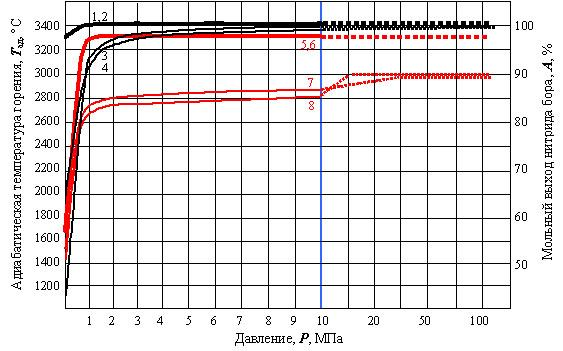
\includegraphics[width=0.8\textwidth]{BN-SHS.png}
%    \caption{Зависимость адиабатической температуры горения систем~СВС}
%    \legend{1,2 – мольный выход BN в системе \ce{4B-3NaN3-NH4Cl}(\ce{NH4Cl}) \\
%        3 – мольный выход BN в системе \ce{8B-3NaN3–KB4} \\
%        4 – мольный выход BN в системе \ce{12B-4NaN3–NH4BF4} \\
%        5 – адиабатическая температура горения в системе \ce{12B - 4NaN3 – NH4BF4} \\
%        6 – адиабатическая температура горения в системе \ce{8B - 3NaN3 – KBF4} \\ 
%       7 – адиабатическая температура горения в системе \ce{4B - NaN3 - NH4Cl}\\
%       8 – адиабатическая температура горения в системе \ce{4B - NaN3 - NH4F}\\
%        }
%    \label{fig:BN-SHS}
%\end{figure}


\begin{figure}[ht]
    \centerfloat{
    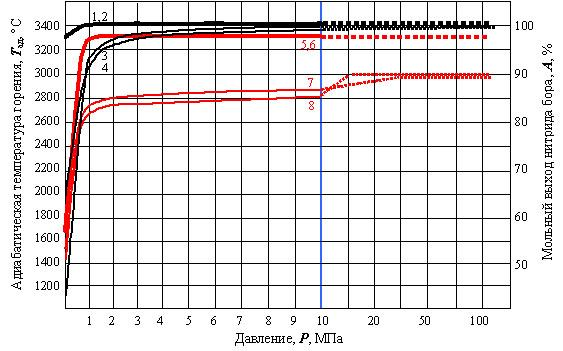
\includegraphics[scale=0.85]{BN-SHS}
    }

 \caption{Зависимость адиабатической температуры горения систем~СВС}\label{fig:BN-SHS}
\end{figure}


\reaction{4B + NaN_3 + Na4Cl -> 4 BN + NaCl + 2H_2}
\reaction{4B + NaN_3 + NH_4F -> 4 BN + NaF + 2H_2}
\reaction{4B + 3NaN_3 + KBF_4 -> 9 BN + 3NaF + KF}
\reaction{12B + 4NaNa_2 + NH_4BF_4 -> 13 BN + NaCl + 2H_2}



\section{Основные виды наноструктур гексагонального нитрида бора}%
\label{sec:Основные виды наноструктур гексагонального нитрида бора}

\cite[]{amos} 

\begin{itemize}
    \item Сферы 
    \item Нанотрубки
    \item Нанолисты
    \item Игольчатые структуры
\end{itemize}

\subsection{Наносферы}%
\label{sub:Наносферы}


\subsection{Нанотрубки}%
\label{sub:Нанотрубки}


Данная структурная модификация BN нашла широкое применение в самых 
различных областях 

\subsection{Нанолисты}%
\label{sub:Нанолисты}

\subsection{Наноиглы}%
\label{sub:Наноиглы}



